%----------------------------------------------------------------------------
\addtocontents{toc}{\protect\newpage}
\chapter{\helm}
%----------------------------------------------------------------------------
A Helm egy olyan eszköz, amely automatizálja a Kubernetes-alkalmazások létrehozását, csomagolását, konfigurálását és telepítését azáltal, hogy a konfigurációs fájlokat egyetlen újrafelhasználható csomagban egyesíti.

Egy mikroszolgáltatás-architektúrában az alkalmazás növekedésével egyre több mikroszolgáltatást hoz létre, ami egyre nehezebben kezelhetővé teszi azt.
A Kubernetes, egy nyílt forráskódú konténer-orchestrációs technológia amely egyszerűsíti a folyamatot azáltal, hogy több mikroszolgáltatást egyetlen telepítésbe csoportosít.
A Kubernetes-alkalmazások kezelése azonban a fejlesztési életciklus során saját kihívások sorát hozza magával, beleértve a verziókezelést, az erőforrás-elosztást, a frissítést és a visszaállításokat.
A Helm az egyik legkönnyebben elérhető megoldást kínálja erre a problémára, következetesebbé, megismételhetőbbé és megbízhatóbbá téve a telepítéseket.

A konténer egy apró szoftverkomponens, amely egy alkalmazást és függőségeit egyetlen képfájlba csomagolja.
A konténerek hordozhatóak a különböző platformok között, ami gyorsabb alkalmazásindítást és egyszerű skálázást eredményez.

A Kubernetes YAML konfigurációs fájlok segítségével telepít.
A gyakori frissítéseket tartalmazó összetett telepítések esetében nehéz lehet nyomon követni ezeknek a fájloknak az összes különböző verzióját.
A Helm egy praktikus eszköz, amely egyetlen telepítési YAML-fájlt tart fenn a verzióinformációkkal.
Ez a fájl lehetővé teszi egy összetett Kubernetes cluster beállítását és kezelését néhány paranccsal \cite{helm}.

\section{Helm chart-ok}
A Helm chart egy olyan csomag, amely tartalmazza az összes szükséges erőforrást egy alkalmazás Kubernetes cluster-re való telepítéséhez.
Ez magában foglalja a telepítésekhez szükséges YAML konfigurációs fájlokat, service-eket, secret-eket és configmap-okat, amelyek meghatározzák az alkalmazás kívánt állapotát.

A Helm chart olyan YAML fájlokat és sablonokat csomagol össze, amelyek segítségével további konfigurációs fájlokat lehet generálni a paraméterezett értékek alapján.
Ez lehetővé teszi a konfigurációs fájlok testreszabását a különböző környezetekhez, valamint újrafelhasználható konfigurációk létrehozását.
Ezenkívül minden egyes chart-ot egymástól függetlenül lehet verziószámozni és kezelni, ami megkönnyíti az alkalmazás több, különböző konfigurációjú verziójának karbantartását \cite{helm}.

\section{Helm működése}
A Helm alkalmazáskönyvtár chart-okat használ a Kubernetes-alkalmazások definiálására, létrehozására, telepítésére és frissítésére.
Ezek a chart-ok lehetővé teszik a Kubernetes manifesztek kezelését anélkül, hogy a Kubernetes parancssori felületéhéz (későbbiekben CLI) hozzá nyúltunk volna vagy bonyolult Kubernetes parancsokat kellene megjegyezni a cluster vezérléséhez.

Tekintsünk egy gyakorlati forgatókönyvet, ahol a Helm hasznos lehet.
Tegyük fel, hogy az alkalmazást tíz replikával rendelkező éles (későbbiekben production) környezetben szeretné telepíteni.
Ezt megadja az alkalmazás telepítési YAML fájljában és a kubectl paranccsal futtatja a telepítést.

Most futtassa ugyanazt az alkalmazást egy tesztelői (későbbiekben staging) környezetben.
Tegyük fel, hogy három replikára van szüksége a staging környezetben, és hogy egy belső alkalmazás buildet fog futtatni a staging környezetben.
Ehhez frissítse a replikák számát és a Docker image taget a telepítési YAML fájlban, majd használja azt a staging Kubernetes cluster-ben.

Ahogy az alkalmazás egyre összetettebbé válik, úgy nő a YAML-fájlok száma is.
Végül a YAML-fájl konfigurálható mezői is megnőnek.
Hamarosan a sok YAML fájl frissítése ugyanazon alkalmazás különböző környezetekben történő telepítéséhez nehezen kezelhetővé fog válni.

A Helm segítségével a mezők a környezettől függően paraméterezhetők.
Az előző példában a replikák és Docker-képek statikus értéke helyett egy másik fájlból veheti át ezeknek a mezőknek az értékét.
Ennek a fájlnak a neve values.yaml \cite{helm}.

\begin{figure}[ht]
    \centering
         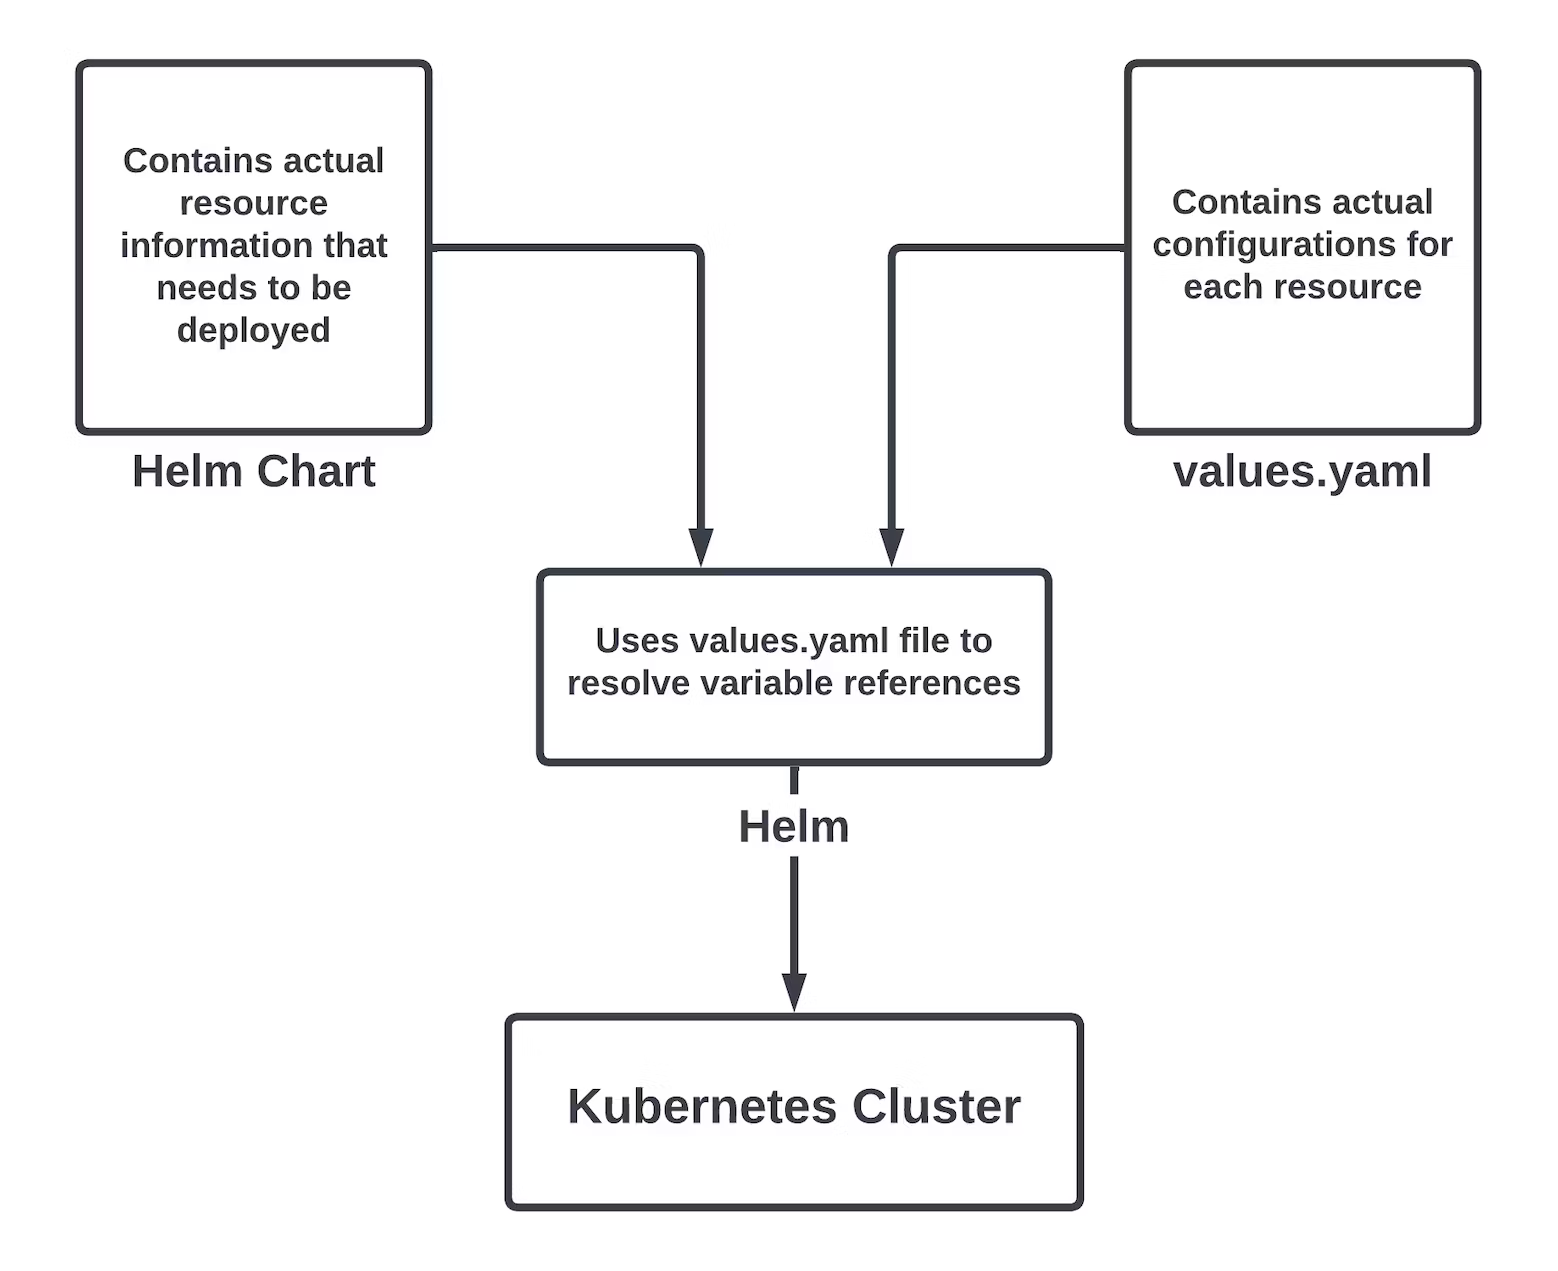
\includegraphics[width=0.9\textwidth]{figures/helm/helm-overview.png}
          \caption{Helm működési folyamatábrája \cite{helm}.}
           \label{helm-overview}
\end{figure}

\section{Helm repository}
A Helm repository az a hely, ahová Helm chart-okat lehet feltölteni.
Létrehozható privát adattár is, ha ez a preferencia.
Az Artifact Hub egy globális Helm adattár, amely kereshető chart-okat tartalmaz, amelyeket számos célra telepíthet.
Röviden, az Artifact Hub azt teszi a chart-ok számára, amit a Docker Hub a Docker-képek számára \cite{helm}.

\section{Mikor érdemes használni}
A Helm akkor hasznos, ha a projekted a Kubernetes segítségével komplex, sok mikroszolgáltatást tartalmazó alkalmazásokat futtat.
A Helm használatával könnyen automatizálható az alkalmazás telepítése és kezelése, csökkentve a kézi munka mennyiségét, és javítva a rendszer megbízhatóságát és stabilitását.
A Helm emellett hozzáférést biztosít az előre konfigurált csomagok kiterjedt tárházához, így könnyen hozzáadható új funkciók az alkalmazáshoz.

Az alkalmazás összetevőinek moduláris táblázatokba szervezésével, amelyeket könnyen telepíthet és frissíthet, a Helm leegyszerűsíti az alkalmazáskomponensek kezelésének folyamatát.
Csökkentheti az alkalmazás karbantartásához szükséges kézi munka mennyiségét, és segít elkerülni a hibákat, amelyek az összetett rendszerek kézi kezelése során keletkezhetnek.

A Helm támogatja a konténerek telepítését több környezetben is, így a konténerek életciklusa a fejlesztési folyamat során könnyen kezelhető \cite{helm}.